  \subsection{Registration and Login System}
Every User who wants to use the application must be registered to the System.
After that, the User has to log in into the System in order to be recognized and use the application.

\begin{table}[H]
	\centering
    
    \begin{tabular}{|p{3.5cm}|p{10.3cm}|}
    
    \hline
    \textbf{\large{Actors}}  			& \tabitem Visitor\\
    				 					& \tabitem Registered User\\
                     					& \tabitem Logged-In User\\
    \hline
    \textbf{\large{Goals}} 				& \ref{goal:trackme1}                                                     \ref{goal:trackme2}\\
    
    \hline
    \textbf{\large{Enter Condition}}	& There is no enter condition for this Use Case		\\
    
    \hline
    \textbf{\large{Events Flow}}		& \begin{enumerate}[leftmargin=0.5cm]
                                          	\item The \emph{Visitor}  accesses to the web site or application log in page
                                            \item The \emph{Visitor} inserts all the mandatory informations (username that will identify the user and password, personal data, email)
                                            \item The System registers the new User and sends back a confirmation email to the provided email address
                                            \item The \emph{Visitor} becomes a \emph{Registered user} inserting a unique username and the password in the log in page   
                                            \item The \emph{Registered User} now can access the \emph{TrackMe} services through the log in page
                                            \item After the insertion of the identifier and password, the \emph{Registered User} becomes a \emph{Logged-in User}
                                          \end{enumerate}
    										\\
    \hline
    \textbf{\large{Exit Condition}} 	& The User is registered in the \emph{TrackMe} System, and his account is added to they system. Now the User is able to use all the functionalities provided by the system. \\
    
    \hline
    \textbf{\large{Exception}} 			& \begin{enumerate}[leftmargin=0.5cm]
                                          	\item The \emph{Visitor} cannot register himself because is already registered.
                                          	\item The \emph{Registered User} is not able to sign in the System because the login data are wrong or he did not confirmed the confirmation email.
                                            \end{enumerate}
    										If one of these problems occur, the system both on the web site and on the application shows a message error to the user, which is invited to re-insert their credentials or confirm the registration email.\\
    
    \hline
    
    \end{tabular}
	
\end{table}
\begin{figure}[H]

    \centering
    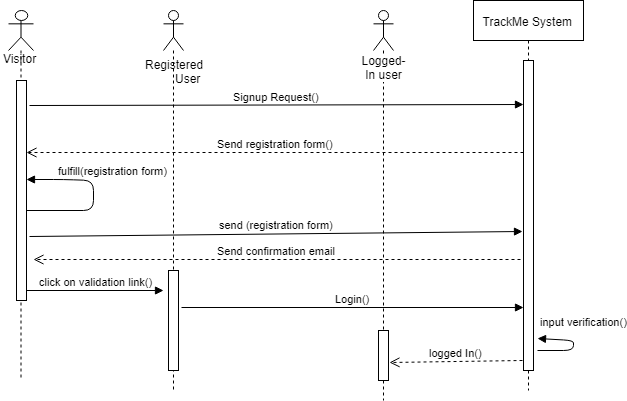
\includegraphics[scale=0.4]{rasdL/Pictures/login1.png}
    \caption{Sequence diagram for the register and login process}
    
\end{figure}

